\documentclass[12pt, a4paper, oneside]{ctexart}
\usepackage{amsmath, amsthm, amssymb, bm, color, graphicx, geometry, hyperref, mathrsfs,extarrows, braket}

\linespread{1.5}
\geometry{left=2.54cm,right=2.54cm,top=3.18cm,bottom=3.18cm}
\newenvironment{problem}{\par\noindent\textbf{题目. }}{\bigskip\par}
\newenvironment{solution}{\par\noindent\textbf{解答. }}{\bigskip\par}
\newenvironment{note}{\par\noindent\textbf{注记. }}{\bigskip\par}

% 基本信息
\newcommand{\dt}{\today}
\newcommand{\sj}{离散数学}
\newcommand{\vt}{吴天阳 2204210460}

\begin{document}

\pagestyle{empty}
\vspace*{-20ex}
\centerline{\begin{tabular}{*3{c}}
    \parbox[t]{0.3\linewidth}{\begin{center}\textbf{日期}\\ \large \textcolor{blue}{\dt}\end{center}} 
    & \parbox[t]{0.3\linewidth}{\begin{center}\textbf{科目}\\ \large \textcolor{blue}{\sj}\end{center}}
    & \parbox[t]{0.3\linewidth}{\begin{center}\textbf{姓名,学号}\\ \large \textcolor{blue}{\vt}\end{center}} \\ \hline
\end{tabular}}
\vspace*{4ex}
\paragraph{习题八}
\paragraph{21.}\begin{solution}
    如下图

    \centerline{
        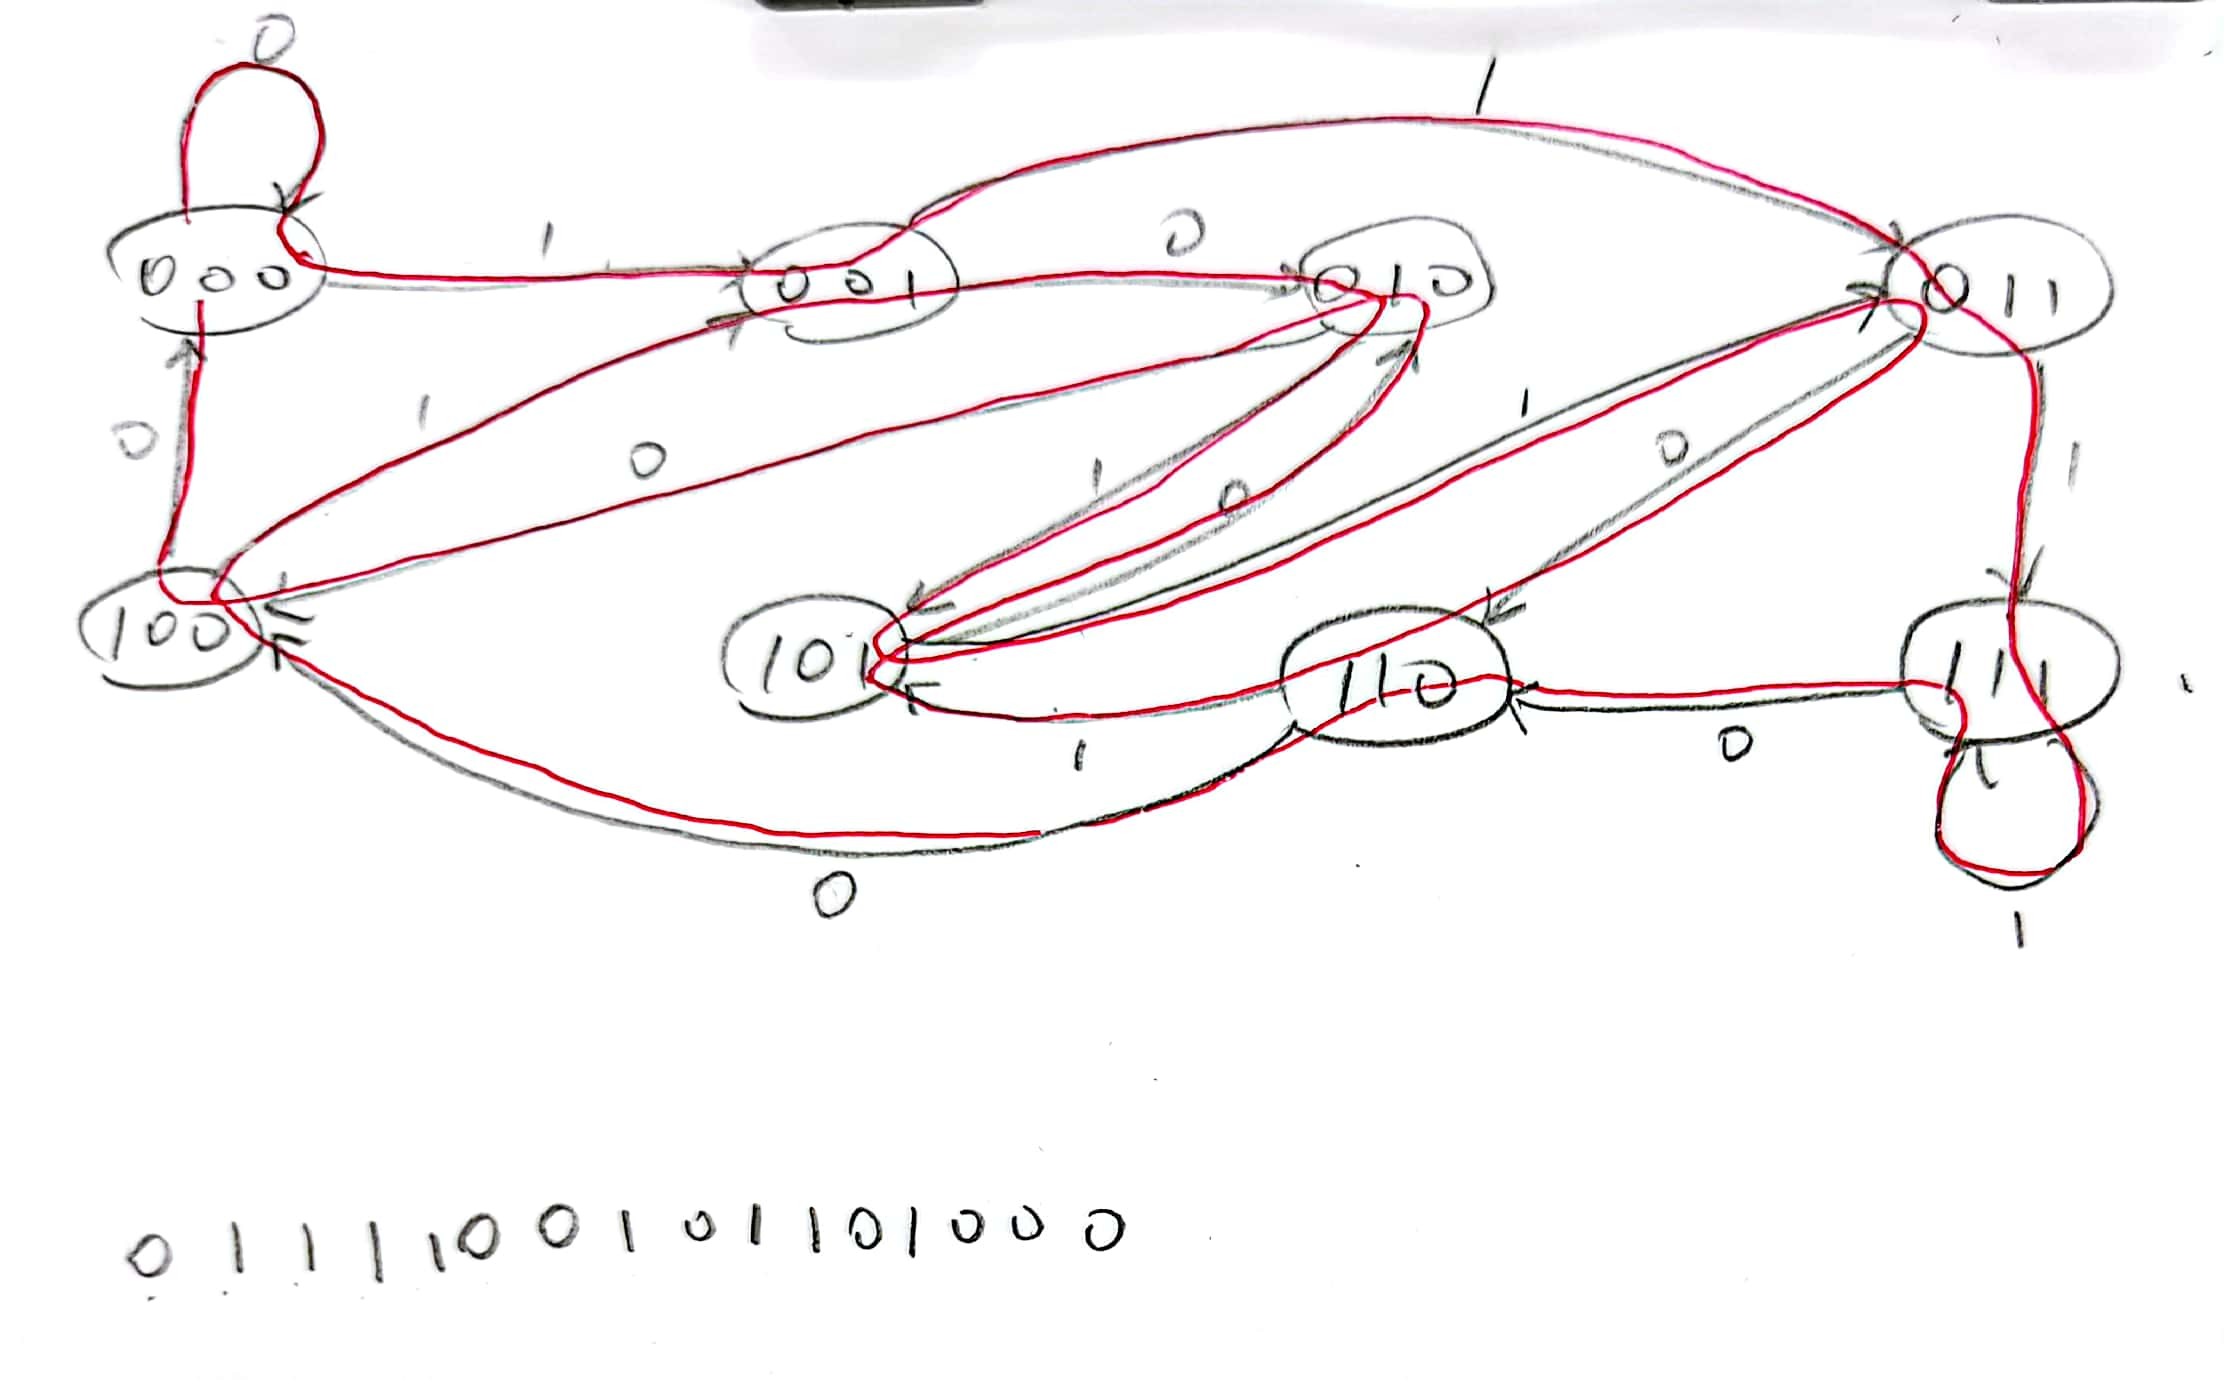
\includegraphics[width=1\textwidth]{graph1.jpg}
    }
\end{solution}
\paragraph{24.}\begin{solution}
    如下图,由于删去$S$集合中的点,导致(a)图中的连通支数为$5 > |S| = 4$,所以(a)图没有$Hamilton$圈。

    由于删去$S$集合中的点,导致(b)图中的连通支数为$8 > |S|+1 = 6+1$,所以(b)图没有$Hamilton$路。

    \centerline{
        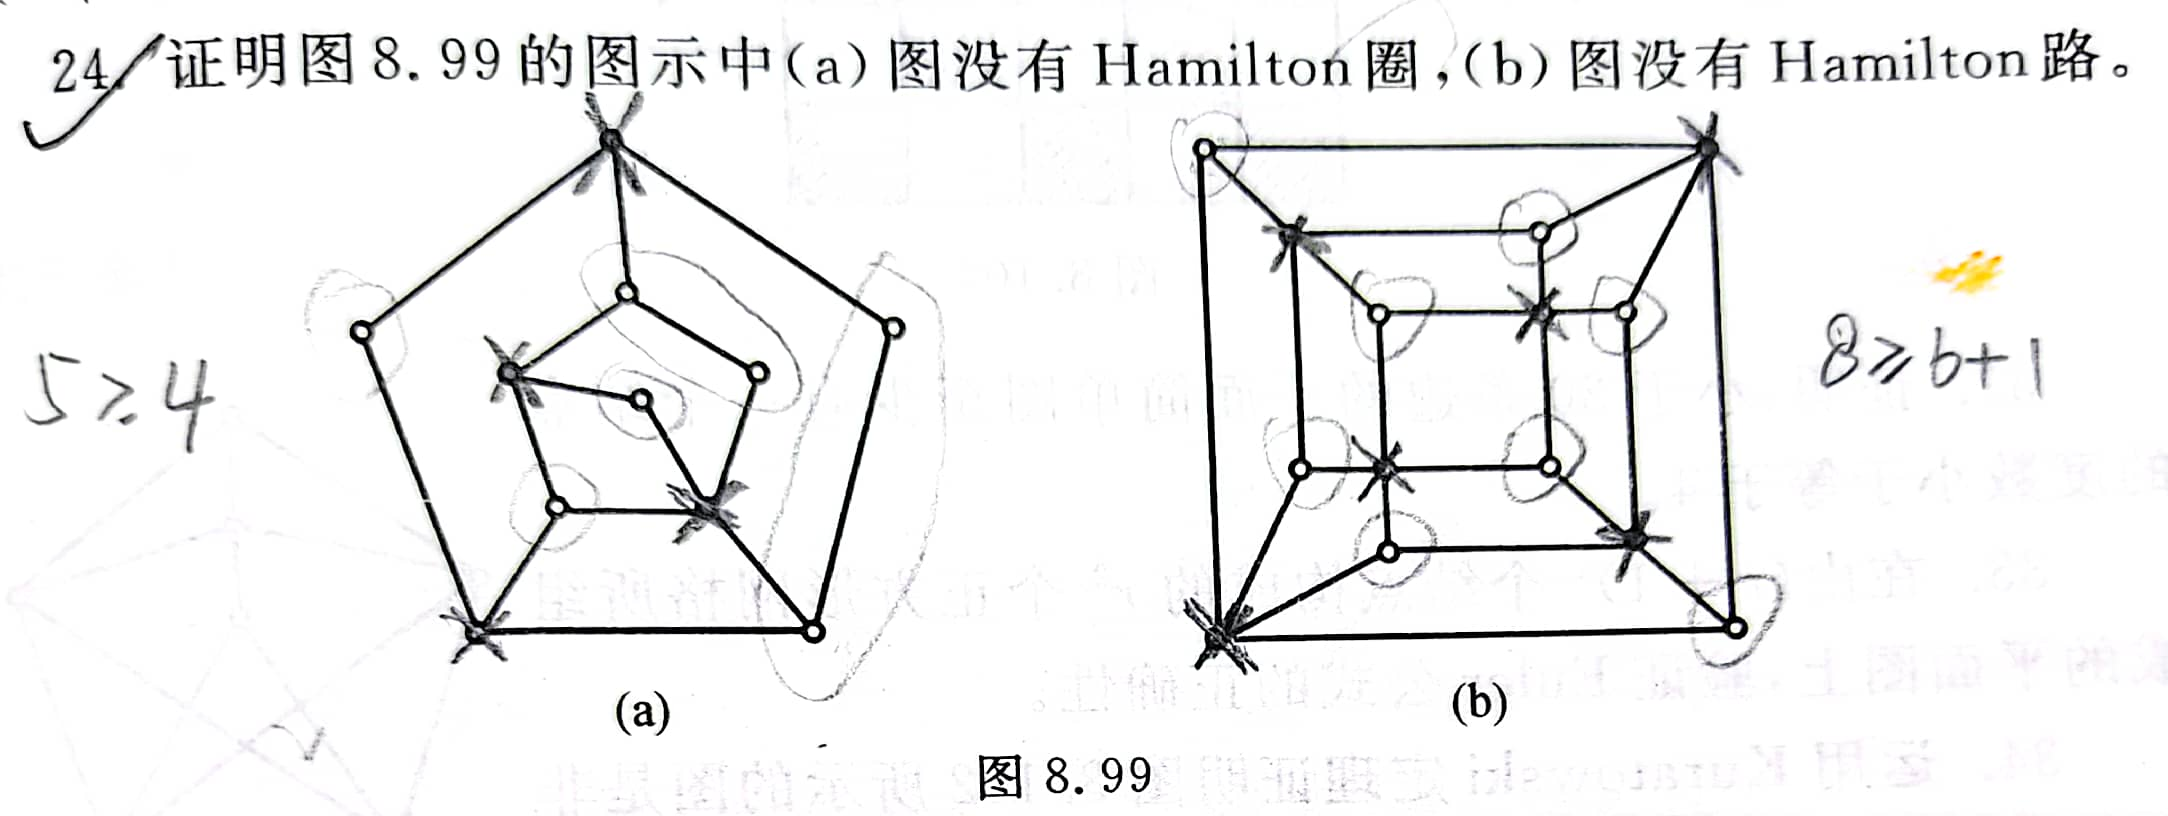
\includegraphics[width=1\textwidth]{graph2.jpg}
    }
\end{solution}
\paragraph{25.}\begin{solution}
    如下图

    \centerline{
        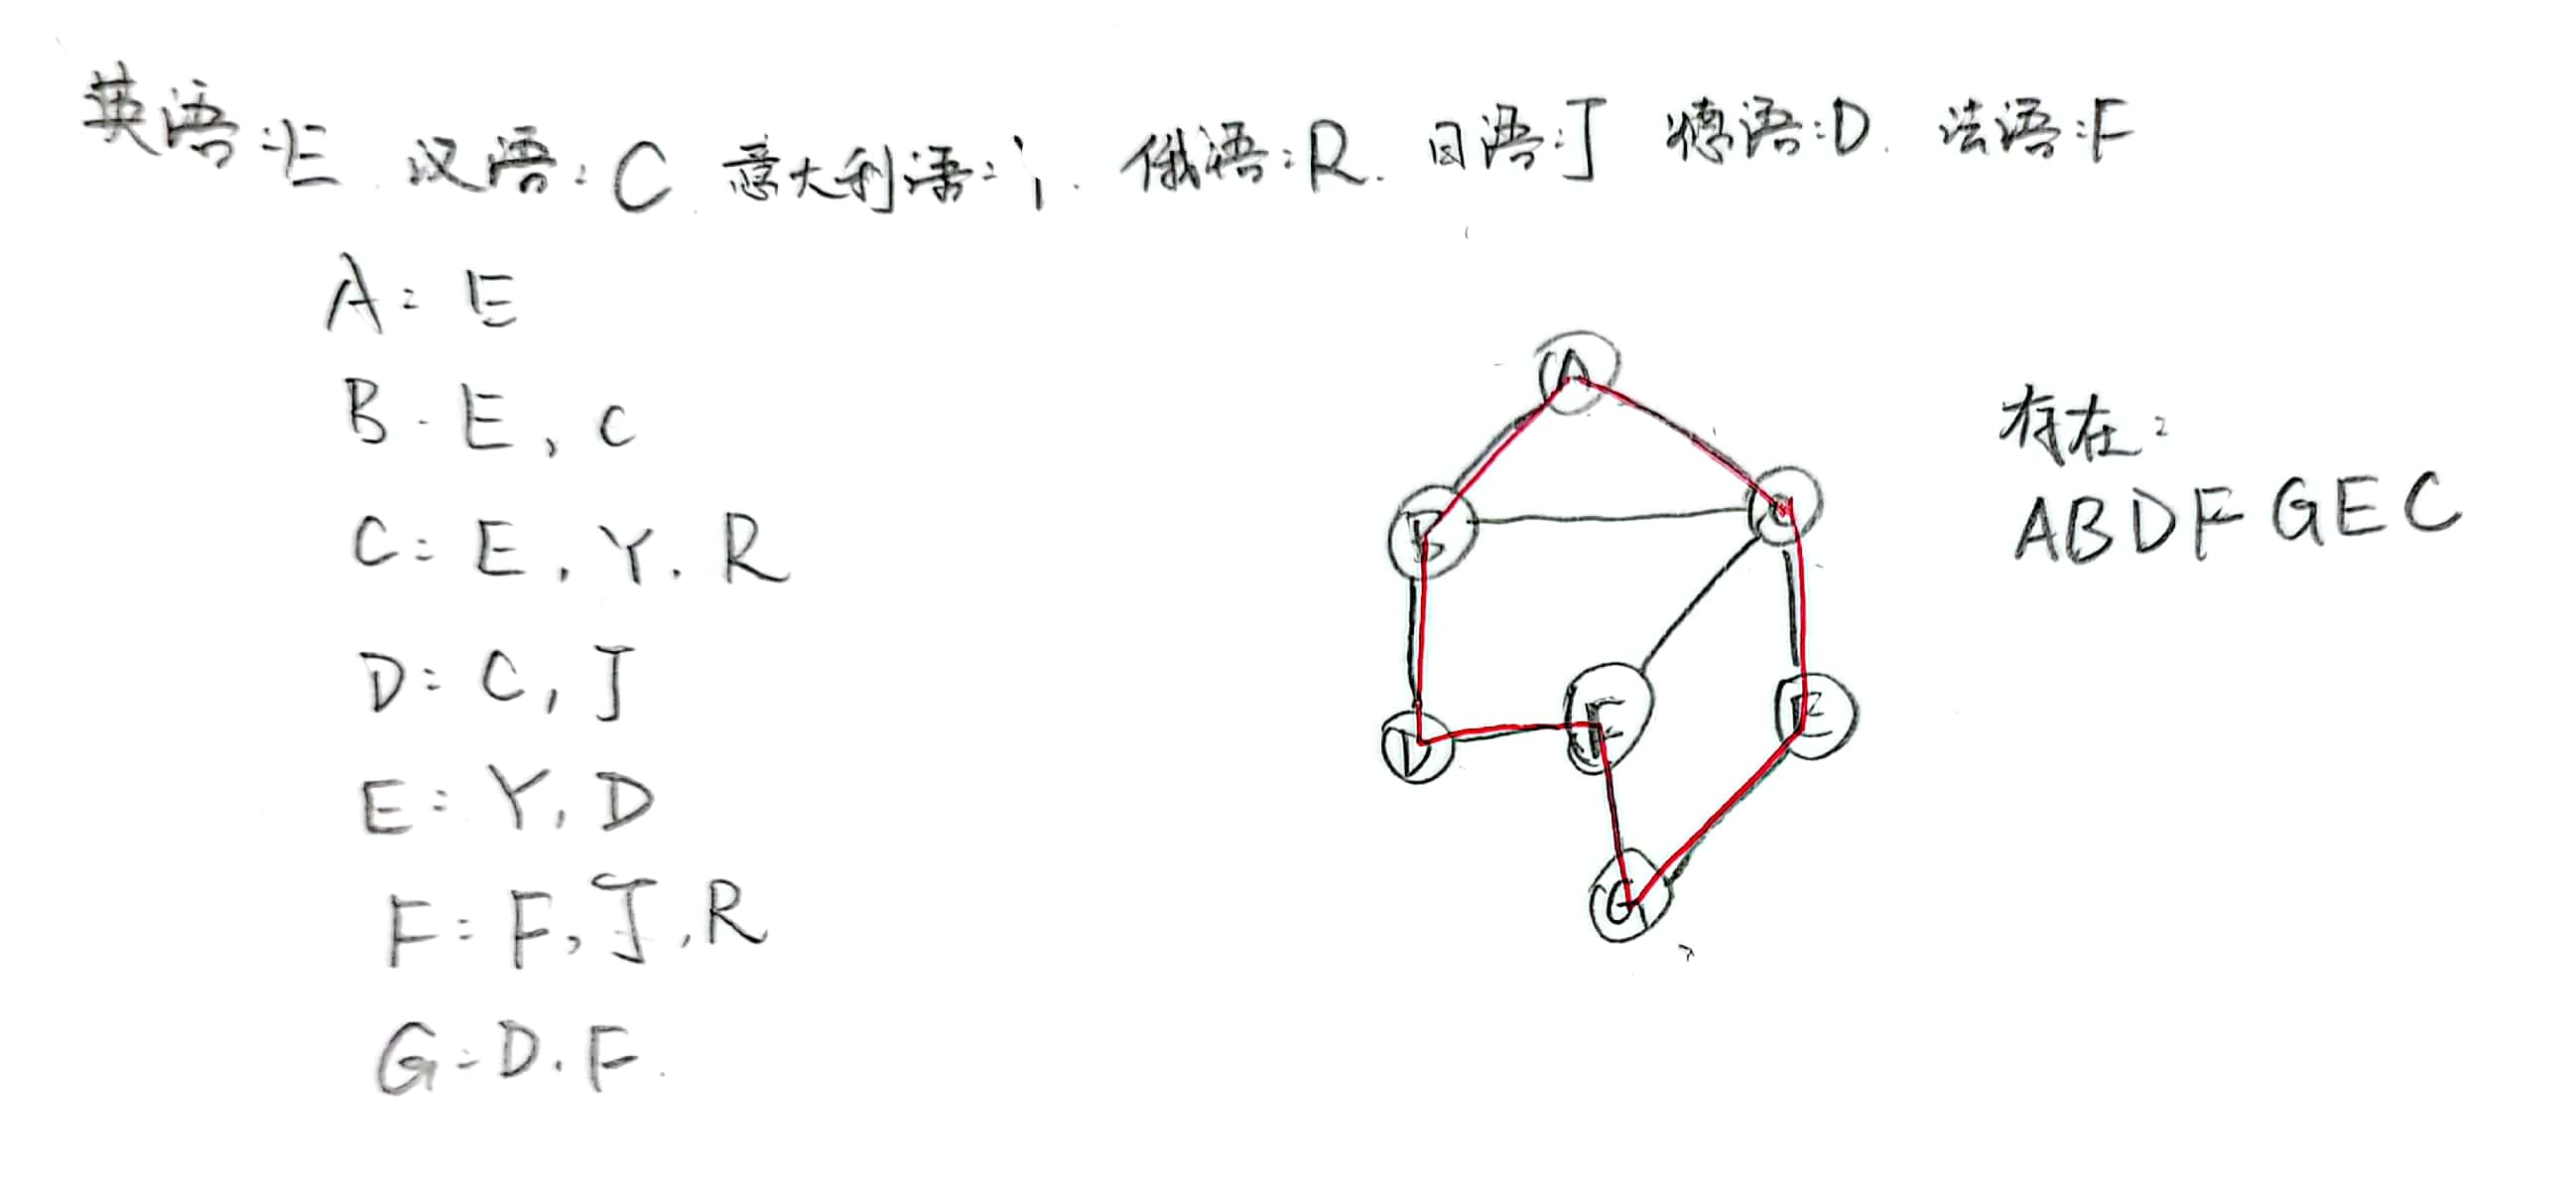
\includegraphics[width=1\textwidth]{graph3.jpg}
    }
\end{solution}
\paragraph{26.}\begin{solution}
    将每个人视为一个点,则一共有$n$个点,如果两个人认识,则在两个人之间连一条边,则对任意的两个结点$u,v$,都有$\text{deg}(u)+\text{deg}(v) \geqslant n-2$,下证利用两个人可以认识其他所有人这个条件可以推出$\text{deg}(u)+\text{deg}(v)\geqslant n-1$,讨论$u,v$之间有无边相连,

    1. $u,v$两个结点间存在连边,则$\text{deg}(u)+\text{deg}(v)=n\geqslant n-1$,命题成立。

    2. $u,v$两个结点间不存在连边,则存在和$v$连接的结点$w$,使得$w$与$u$之间没有连边,对于结点$v,w$,由于$u$结点都没有直接连边,所以他们合起来也不认识$u$与条件矛盾。

    综上,对于任意两个结点$u,v$,有$\text{deg}(u)+\text{deg}(v)=n\geqslant n-1$成立,所以图中存在一个$Hamilton$路,使得所有人按照该路径排成一条,满足题意。
\end{solution}
\paragraph{28.}\begin{proof}
    设二分图$G$对所有结点划分为$n_1,n_2$个结点,则$n_1+n_2 = n$,由于$G$为二分图,则$m\leqslant n_1n_2=(n-n_2)n_2$,由于当$n_2=\dfrac{n}{2}$时,$(n-n_2)n_2$有最大值为$\dfrac{n^2}{4}$,故
    \begin{equation*}
        m\leqslant \frac{n^2}{4}
    \end{equation*}
\end{proof}
\paragraph{30.}\begin{solution}
    不存在完美匹配,因为总结点数为奇数个,故不存在匹配$M$,使得$|M|=|V_1|=|V_2|$成立。

    利用贪心的思路,容易看出一个最大匹配:
    \begin{equation*}
        M = \{(v_1,u_2),(v_2,u_1),(v_3,u_4),(v_4,u_3)\}
    \end{equation*}
\end{solution}
\paragraph{31.}\begin{solution}
    不存在这样的路线,因为,如果走完$25$间房间,一共移动$24$次,为偶数次,由于每移动一次颜色发生变化,所以入口的颜色与出口的颜色必定相同,而该题入口与出口颜色不同,所以一定不存在这样的路径。
\end{solution}
\end{document}
